\section{Zielsetzung}
\label{sec:Zielsetzung}
Ziel ist es, die Leerlaufspannung und den Innenwiderstand unterschiedlicher
Spannungsquellen zu messen.

\section{Theorie}
\label{sec:Theorie}
Wird einer Spannungsquelle kein Strom entnommen, so liegt an den Ausgangsklemmen
die Leerlaufspannung $U_\text{0}$ an. Wird in den Schaltkreis ein Lastwiderstand
$R_\text{a}$ geschaltet, fließt ein endlicher Strom $I$ und die Klemmenspannung
$U_\text{K}$, welche an einer belasteten Spannungsquelle abgegriffen werden kann,
sinkt auf einen Wert unterhalb $U_\text{0}$ ab. Der Spannungsquelle wird also ein
Innenwiderstand $R_\text{i}$ zugeordnet. Aufgrund des Zweiten Kirchhoff'schen Gesetzes gilt
für solch einen Schaltkreis (Abbildung 1)

%Kirchhoff2
\begin{align*}
U_\text{0} = I R_\text{i} + I R_\text{a}.
\end{align*}

%Schaltung Theorie
\begin{figure}
  \centering
  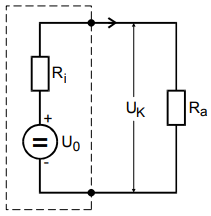
\includegraphics{schalt1.png}
  \caption{Ersatzschaltbild einer realen Spannungsquelle $U_\text{0}$ mit 
  Innenwiderstand $R_\text{i}$ und Lastwiderstand $R_\text{a}$. \cite[S. 1]{l}}
  \label{fig:schaltung1}
\end{figure}

Da
\begin{align}
U_\text{K} = I R_\text{a} = U_\text{0} - I R_\text{i}
\end{align}
gilt, ist es sinnvoll zur Messung der Leerlaufspannung den Widerstand 
$R_\text{a}$ des Messgerätes so groß wie möglich zu halten. Wegen des
daraus resultierend geringen Stromes kann so
\begin{align*}
U_\text{K} \approx U_\text{0}
\end{align*}
angenommen werden. Der Innenwiderstand $R_\text{i}$ bewirkt auch, dass einer
idealen Spannungsquelle nicht unendlich elektrische Leistung entnommen werden kann.
Die an $R_\text{a}$ abgegebene Leistung lässt sich mit
\begin{align}
N = I^{2} R_\text{a}
\end{align}
bestimmen. Bei der Leistungsanpassung wird ein $R_\text{a}$ gewählt, bei dem $N$
maximal wird. Bei elektrischen Generatoren ist der Innenwiderstand nicht durch 
Gleichstromwiderstand, sondern durch einen Rückkopplungsmechanismus festgelegt.
Ändert sich also der Belastungsstrom, so ändert sich auch das elektrische Verhalten
von diesem, sodass der Innenwiderstand als differentielle Größe
\begin{align*}
R_\text{i} = \frac{dU_\text{K}}{dI}
\end{align*}
eingeführt wird.